\newpage
\section{Concepts Considered}

% Need to talk about which concepts we took, and refer to the brainstorm idea.

Following extensive brainstorming and analysis, our team carefully evaluated a wide range of potential features and implementation strategies for our smart lock system. Ultimately, we selected the concept of using a solenoid-based locking mechanism controlled via a keypad and a smartphone app. This approach balanced feasibility, security, and user convenience. Our selection process included the use of the 6-3-5 method, which helped generate and refine a wide range of ideas across five categories: Hardware \& Mechanics, Smartphone Integration, Security Features, Software \& Control, and Advanced Features. We also brainstormed ideas of how the lock would potentially look like, for easy installation and fix up when an issue arises. 

% Refer to the appendix sections for 635, brainstorming, morphological charts, mind maps

\subsection{6-3-5 Method}
\subsubsection*{Hardware \& Mechanics}
\begin{itemize}
    \item use a servo motor for deadbolt control
    \item hall effect sensor to detect if the door is open or closed
    \item implement linear actuator for silent locking
    \item maybe anti-backlash gears to reduce mechanical play
    \item consider designing a modular lock housing with 3D-printed parts
    \item have a backup battery to ensure operation during power outages
\end{itemize}

\subsubsection*{Smartphone Integration}
\begin{itemize}
    \item develop a smartphone app for remote locking/unlocking
    \item push notifications for lock activity (ex: ``Door locked at 3:45 PM'')
    \item have biometric authentication (Face ID or fingerprint)
    \item Use Bluetooth for proximity-based auto-unlock
    \item NFC support for quick unlocking via phone tap
    \item include multi-user access control with time-based permissions
\end{itemize}

\subsubsection*{Security Features}
\begin{itemize}
    \item Implement AES-256 encryption for communication between the lock and phone
    \item maybe two-factor authentication for app access
    \item develop a tamper-detection alarm if the lock is forced
    \item lockdown mode for multiple failed attempts
    \item include a manual override mechanism in case of system failure
    \item utilize rolling codes for Bluetooth pairing to prevent hacking
\end{itemize}

\subsubsection*{Software \& Control}
\begin{itemize}
    \item ESP32 microcontroller for Wi-Fi and Bluetooth control
    \item Develop a closed-loop system to verify if the lock is engaged properly
    \item make a real-time event log accessible via the app
    \item add a scheduling feature for auto-locking at specific times
    \item guest mode with temporary passcodes
    \item Integration with voice assistants like Alexa or Google Assistant
\end{itemize}

\subsubsection*{Advanced Features}
\begin{itemize}
    \item GPS stuff
    \item add geofencing to lock or unlock based on the user's location
    \item integrate with smart home platforms like Home Assistant
    \item use AI-based behavior analysis to suggest locking patterns
    \item add a camera with facial recognition for auto-unlock
    \item enable remote firmware updates
    \item learn database SQL
    \item use solar charging for battery-powered locks
\end{itemize}



% BRAINSTORMING -----------------------------




\subsection{Brainstorming}

\subsubsection*{Adam Wu}
\begin{itemize}
    \item As a person who has amnesia, I would like to be able to find my keys anytime so that when I forget where I place them, I can find them.
    \begin{itemize}
        \item Having a "find my" solution with a key.
    \end{itemize}
    \item As a person who loves security, I would like to have the best lock for my house so that lock pickers are not able to pick my lock.
    \begin{itemize}
        \item Making an “authentication” key that resets the key code within a set time, making it harder for hackers to unlock the door.
    \end{itemize}
    \item As a person who is always last-minute out the door, I fear forgetting to lock the door when I close it.
    \begin{itemize}
        \item Auto-locking door when a person closes the door.
    \end{itemize}
    \item As a person who often forgets to bring their keys, I am scared of getting locked out.
    \begin{itemize}
        \item Having a notification from the key to the phone that alerts: “keys are not close by to you.”
    \end{itemize}
    \item As a parent, I am scared of my kids forgetting their keys and locking themselves out of their room.
    \begin{itemize}
        \item Creating a “master key” that only parents/admins can use to unlock specific doors.
    \end{itemize}
    \item Concerned about key battery life.
    \begin{itemize}
        \item Send a notification to the user when the key is on low battery.
    \end{itemize}
\end{itemize}

\subsubsection*{Nathaniel Laurente}
\begin{itemize}
    \item Key has the ability to notify the user when too far away from the user’s phone/body.
    \item Key deactivates/won’t be able to open the door if too far away from the owner.
    \item “Tap to Pay” technology concept.
    \begin{itemize}
        \item Unlocks the door like a credit card tap on a phone.
        \item If too complex, explore alternative ways to unlock the door.
        \item Eliminates the need for a physical key.
        \item Prevents stolen keys from working if the user still has their phone.
    \end{itemize}
    \item Secure deactivation of the key when too far from the user.
    \begin{itemize}
        \item Possible solution: Use the user's phone for deactivation.
    \end{itemize}
    \item One-time password generator between lock and key to ensure only this exact key can enter the house.
    \item Backup way to get into the house if the user forgets/loses their key.
    \begin{itemize}
        \item Pin access code.
        \item App allows for 2FA authentication using a thumbprint and/or Face ID.
    \end{itemize}
    \item Will the battery last long enough for multiple years?
\end{itemize}

\subsubsection*{Neena Nguyen}
\begin{itemize}
    \item Existing smart lock solutions:
    \begin{itemize}
        \item Smart locks for dorm rooms using mobile apps, passcodes, and scanners.
    \end{itemize}
    \item Who will use this lock?
    \begin{itemize}
        \item People with memory issues (elderly, ADHD).
        \item University students in dorm rooms.
        \item Student ID scanner integration.
        \item Parents with small children (child-proof locks).
    \end{itemize}
    \item Features for parental control.
    \begin{itemize}
        \item Locks after a curfew time.
        \item Prevents children from unlocking without parental approval.
        \item Alerts parents when kids come home from school.
    \end{itemize}
    \item What kind of door lock will it be?
    \begin{itemize}
        \item Facial recognition (requires camera and database knowledge).
        \item Logs entry and exit timestamps.
        \item Digital passcode through an app.
        \item Auto-relocking mechanism after failed attempts.
        \item Bluetooth detection for unlocking within a certain range.
        \item Dual authentication (PIN + scan).
        \item Optional security trigger after specific hours.
        \item Alerts when the door is left unlocked for too long.
        \item Auto-locking after prolonged unlocking.
        \item Detection system to check if the key is on the person.
        \item Prevents intruders from entering without a key.
    \end{itemize}
\end{itemize}

\subsubsection*{Jackson Kennedy}
\begin{itemize}
    \item Normal keys can be lock-picked, but digital keys can be secured based on a communication protocol.
    \item Secure authentication methods.
    \begin{itemize}
        \item PIN authentication with 2FA.
        \item Optimal PIN length (e.g., 4-digit PIN has 1,048,576 combinations).
        \item Brute force prevention strategies.
    \end{itemize}
    \item Preventing communication protocol vulnerabilities.
    \begin{itemize}
        \item What protocol should be used? (Bluetooth has vulnerabilities and short range.)
        \item Cloud-based solutions rely on third-party vendor security.
        \item What information needs to be transferred? (Video data, authentication signals?)
    \end{itemize}
    \item Lock activation logic.
    \begin{itemize}
        \item How exactly will the lock know when to unlock? (Sending a 0 or 1 signal based on specific conditions?)
    \end{itemize}
    \item Security and alerting technologies.
    \begin{itemize}
        \item Sensors to detect nearby people.
        \item Hidden camera or biometric verification for identity confirmation.
    \end{itemize}
    \item Scheduling and timed access.
    \begin{itemize}
        \item Physical locks do not have scheduling options.
        \item Implement timed unlocking (e.g., unlock for 15 minutes for a babysitter).
        \item Extra verification to prevent intruders from exploiting schedules.
    \end{itemize}
\end{itemize}
\newpage









% Begin Morphological Charts ----------------------------------

\subsection{Morphological Charts}

\begin{figure}[!ht]
    \centering
    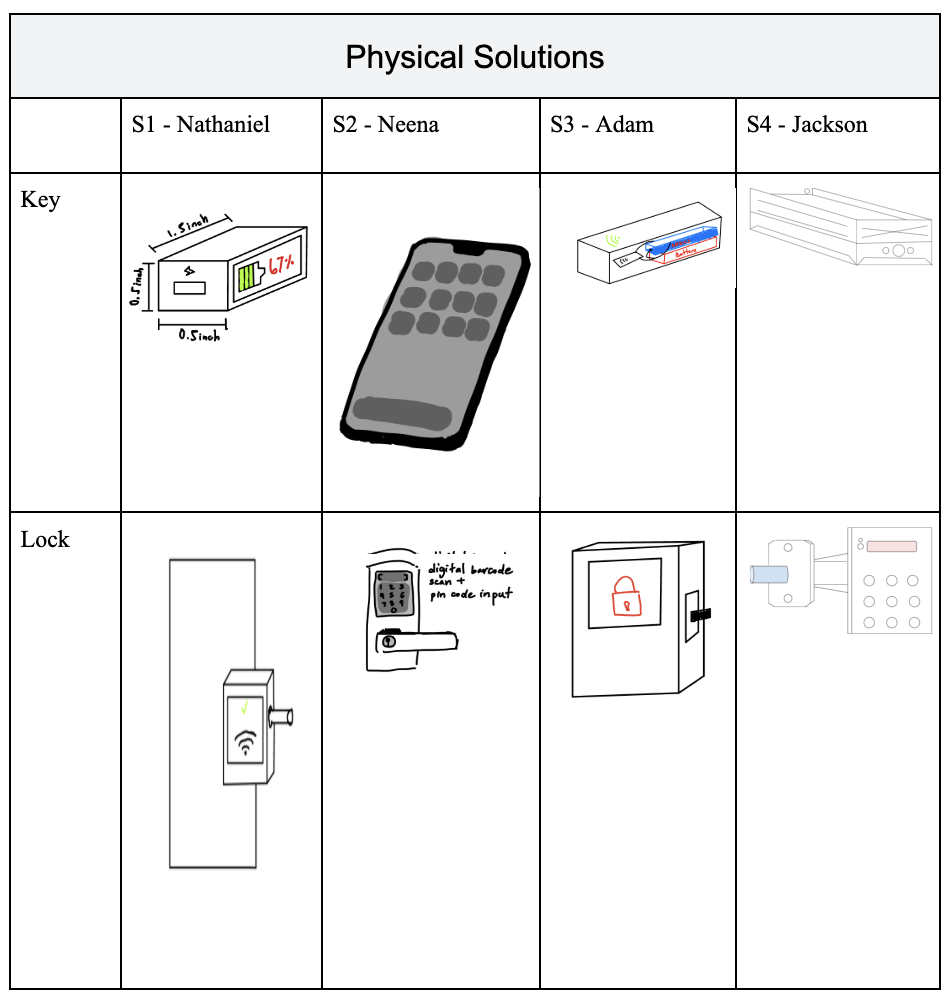
\includegraphics[width=1\linewidth]{./img/p1mm.png}
    \caption{Physical Solution Chart}
    \label{fig:p1mm}
\end{figure}
\newpage
\begin{figure}[!ht]
    \centering
    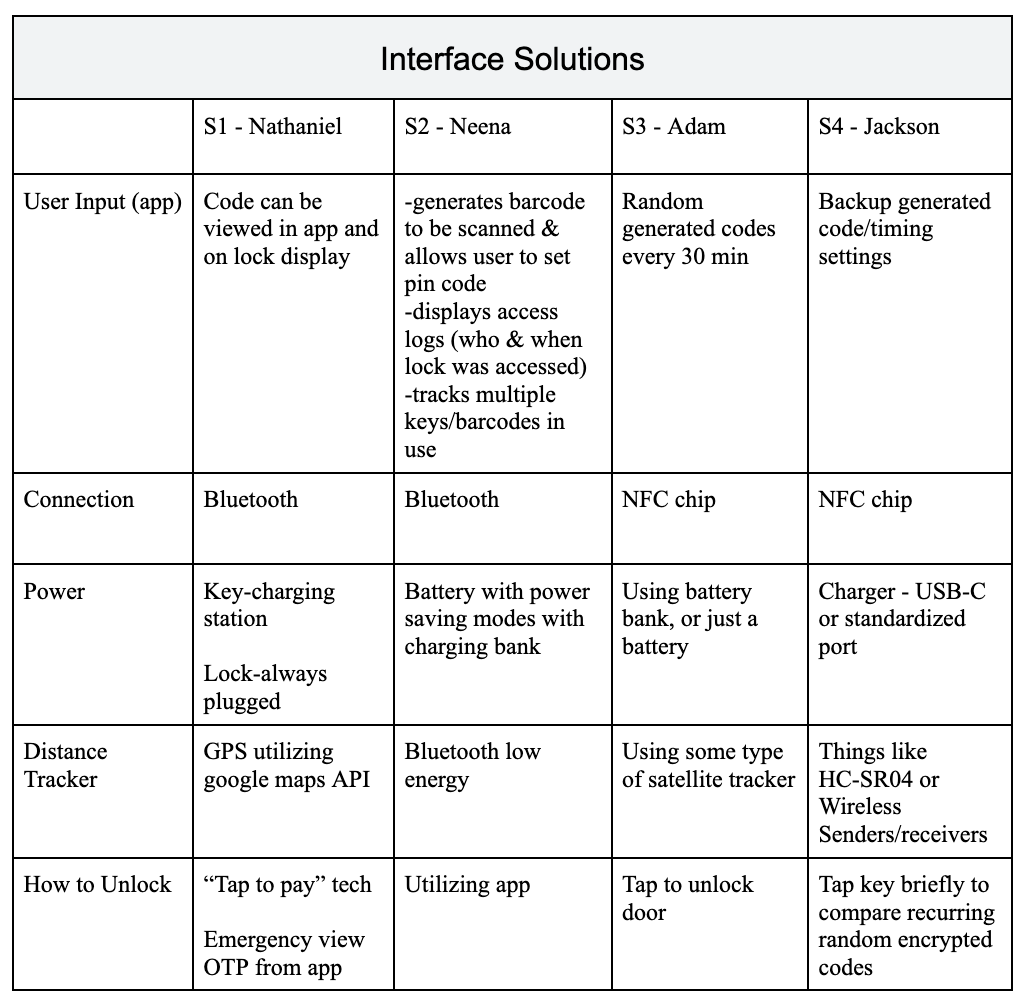
\includegraphics[width=1\linewidth]{./img/p2mm.png}
    \caption{Interface Solutions}
    \label{fig:p2mm}
\end{figure}
\newpage





% Begin Mind Map ---------------------------------------------

\subsection{Mind Map}

\begin{figure}[!ht]
    \centering
    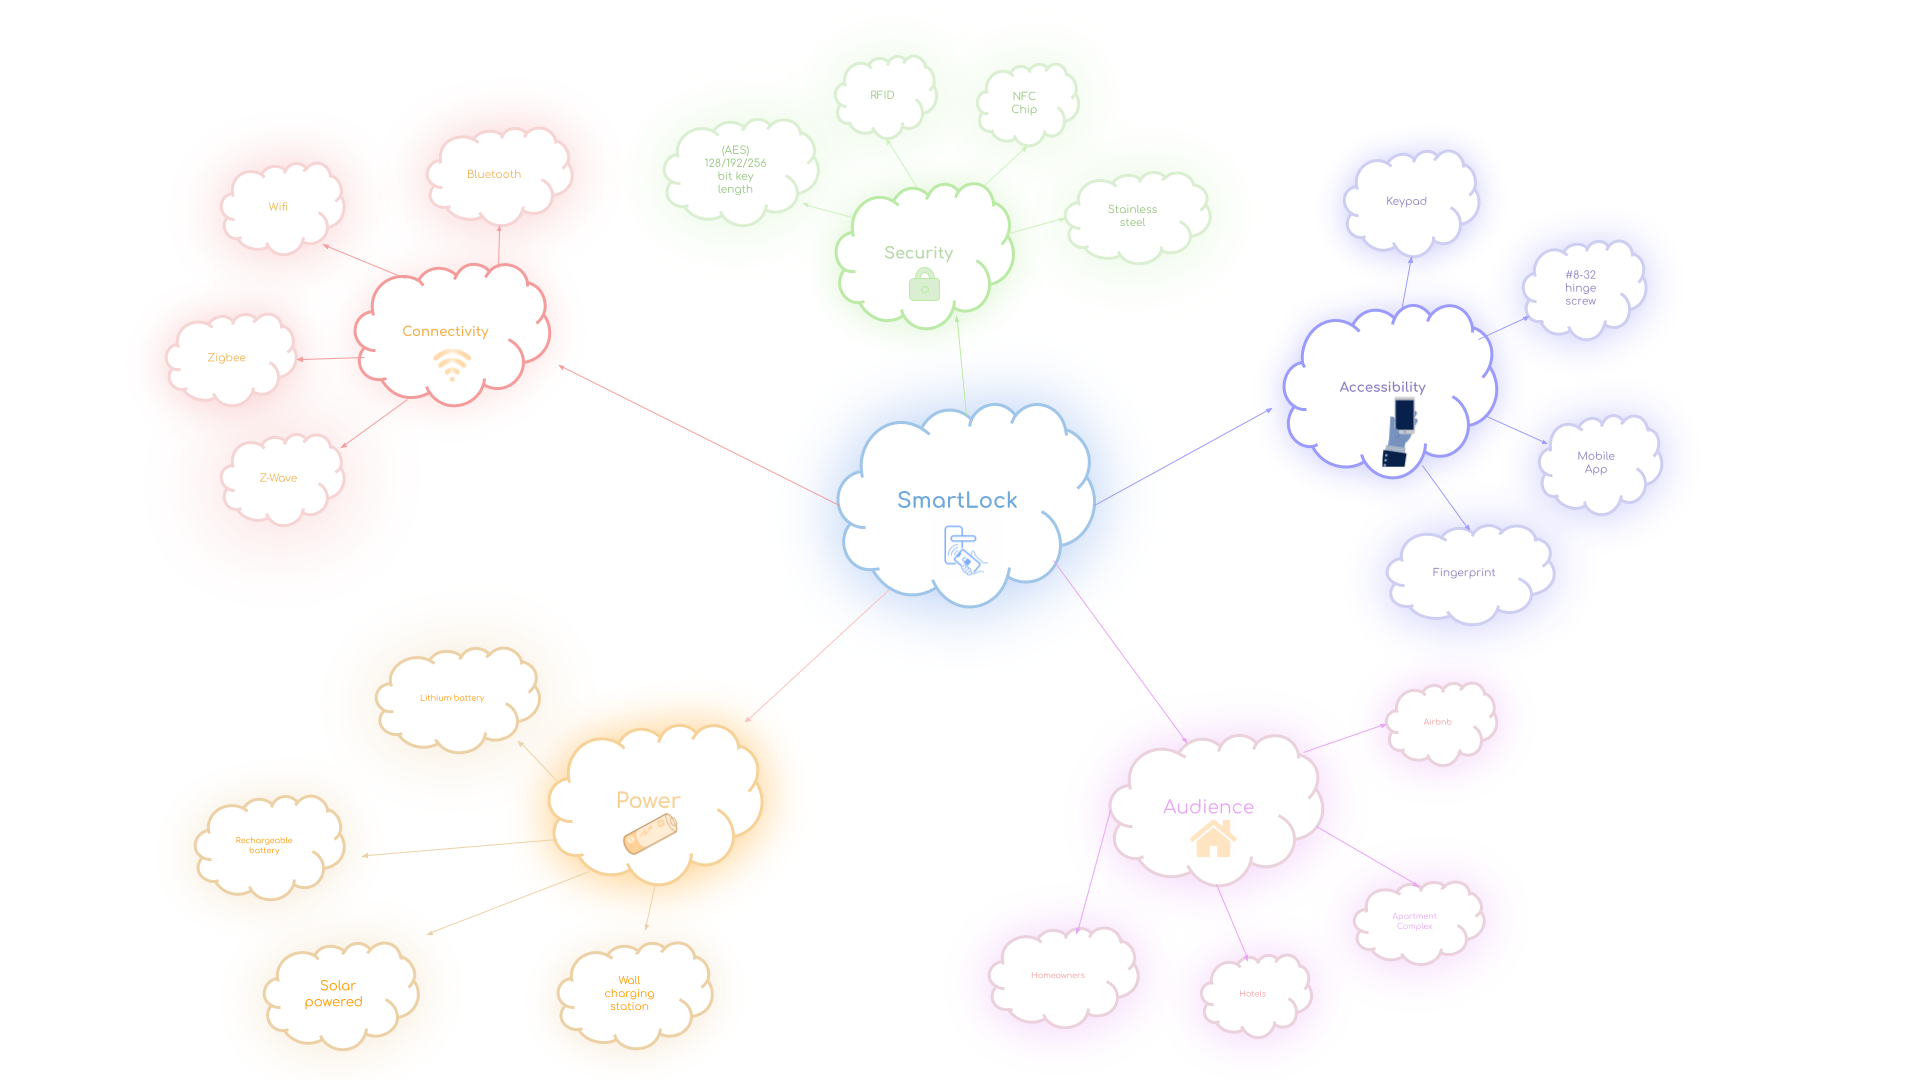
\includegraphics[width=140mm,scale=0.5]{./img/mindmapsmartlock.png}
    \caption{Mind Map}
    \label{fig:mindmapsmartlock}
\end{figure}
\newpage